%!TEX options = --shell-escape


\documentclass[master]{thesis-uestc}
\title{基于图同构的数学推理引擎的设计与实现}                                   %论文标题
\titleEn{A Research of Multi-function Switched-beam Antenna Array} %英文标题
\author{李菲}                                                      %作者
\authorEn{Li Fei}                                               %作者英文名
\advisor{符红光 \hspace{0.2in} 教授}                                  %导师
\advisorEn{Prof. Li Si}                                            %导师师英文名
\school{School of uestc}                                        %学院英文名
\major{理学硕士}                                            %专业
\majorEn{Master of Pharmacy}           %专业英文名
\studentid{201852081006}
\usepackage{makecell}

\begin{document}
\makecover  %封面

% abstract
\documentclass{standalone}
% preamble: usepackage, etc.
\begin{document}
	
\begin{chineseabstract}
近些年,人工智能已经由传统的感知智能逐渐向认知智能阶段过渡,认知智能与自动推理成为很多专家学者
以及科研机构研究的重点。目前是处于认知智能发展的初期,面临着诸多挑战的同时也伴随着机遇。如何
将深度学习应用于逻辑推理,从而让机器具备思考和推理能力将是人工智能重大突破口。本文的研究内容是
基于图同构的初等数学推理引擎的设计和构建,推理引擎是整个自动推理系统最核心的部分。推理引擎的
系统设计理念是基于产生式系统,同样涉及到知识表示和实例化规则库构建两部分。具体研究内容如下:

(1)初等数学的知识表示

知识表示是类人解答系统求解问题的第一步,只有先将人类的语义转换成计算机的知识结构,才能进行后续的推理和
问题求解工作。知识表示的方法多种,由于本文研究课题对象是初等数学问题,分析和总结初等数学的知识具有概念
清晰严谨、定理明确以及公式化程度高等特点,最终选用知识图谱来表示数学中概念实体和它们之间的关系在实际编码中使用Java中的类结构来构建
初等数学的实体类和关系类,为了知识图谱构建的可扩展性和开闭性原则,选用抽象类的继承思想去扩展,即
所有的实体类都继承于抽象实体类,所有的关系类都继承于抽象关系类。

(2)构建实例化定理库

基于产生式系统的推理引擎,规则库是引擎重要的外部驱动和产生知识的依据。本文构建的规则库也是知识图谱的
方式表示和存储。实例化定理库的构建分为三个步骤:定理来源、定理标准化以及定理实例化。首先定理来源于
教材和教辅中的公式定理,以及标准答案的解答过程、解题技巧。对于搜索的定理是需要转换成推理引擎统一的
格式,这个过程叫定理标准化,方便推理引擎简单统一。最后将标准化定理生成知识图谱完成实例化。

(3)图同构的推理引擎的设计和构建
本文的推理引擎设计思想上可以从三个不同的角度去理解。首先是引擎中推理系统设计模式,是基于”先逆后正“
逻辑的产生式系统,并设计成逻辑推理与计算推理交互推理的混合推理;其次,从引擎逻辑结构考虑,引擎采用分层
结构,每个逻辑层之间保持相对独立性;最后,考虑引擎核心算法的设计,图匹配的算法思想在于是一种混合匹配算法,
知识图谱上通过类型匹配构建实体和关系的映射,然后再对字符串做模式匹配,生成符号轮换集。

本文完成了基于图同构的数学推理引擎的整个算法设计和所有模块的构建工作,完成非应用题的随机
批量测试和高考试卷测试,综合解题率71.2\%,平均求解时间不超过5分钟。


\chinesekeyword{认知智能,图匹配推理引擎,符号计算,类人解答系统,知识表示,实例化定理}
\end{chineseabstract}

\end{document} %中文摘要
\documentclass{standalone}
% preamble: usepackage, etc.
\begin{document}

\begin{englishabstract}
	With the widespread engineering applications ranging from broadband signals and non-linear systems, time-domain integral equations (TDIE) methods for analyzing transient electromagnetic scattering problems are becoming widely used nowadays. TDIE-based marching-on-in-time (MOT) scheme and its fast algorithm are researched in this dissertation, including the numerical techniques of MOT scheme, late-time stability of MOT scheme, and two-level PWTD-enhanced MOT scheme. The contents are divided into four parts shown as follows.
	
	\englishkeyword{time-domain electromagnetic scattering, time-domain integral equation (TDIE), marching-on in-time (MOT) scheme, late-time instability, plane wave time-domain (PWTD) algorithm}
\end{englishabstract}

\end{document}
 %英文摘要

% table of contents
\thesistableofcontents   %目录
% thesis contents
\documentclass{standalone}
% preamble: usepackage, etc.
\begin{document}

\thesischapterexordium

\section{研究工作的背景与意义}
人工智能(Artificial Intelligence,AI)作为研究、开发用于模拟和扩展人类智能的理论、方法以及技术
和应用系统的一门新兴科学\citing{sun2013ren}。人工智能的概念1956年的研讨会正式被提出开始,它的发
展可谓是起起落落充满曲折坎坷。时至今日,人工智能在科研、教育、医疗、金融等各方面正大放异彩。无论
是理论还是应用层面都取得了不错的进展。

%计算电磁学方法\citing{wang1999sanwei, liuxf2006, zhu1973wulixue, chen2001hao, gu2012lao, feng997he}从时、频域角度划分可以分为频域方法与时域方法两大类。频域方法的研究开展较早,目前应用广泛的包括:矩量法(MOM)\citing{xiao2012yi,zhong1994zhong}及其快速算法多层快速多极子(MLFMA)\citing{clerc2010discrete}方法、有限元(FEM)\citing{wang1999sanwei,zhu1973wulixue}方法、自适应积分(AIM)\citing{gu2012lao}方法等,这些方法是目前计算电磁学商用软件
%\footnote{脚注序号“\ding{172},……,\ding{180}”的字体是“正文”,不是“上标”,序号与脚注内容文字之间空1个半角字符,脚注的段落格式为:单倍行距,段前空0磅,段后空0磅,悬挂缩进1.5字符;中文用宋体,字号为小五号,英文和数字用Times New Roman字体,字号为9磅;中英文混排时,所有标点符号(例如逗号“,”、括号“()”等)一律使用中文输入状态下的标点符号,但小数点采用英文状态下的样式“.”。}
%(例如:FEKO、Ansys 等)的核心算法。由文献\citing{feng997he, xiao2012yi, clerc2010discrete}可知

\section{时域积分方程方法的国内外研究历史与现状}
时域积分方程方法的研究始于上世纪60 年代,C.L.Bennet 等学者针对导体目
标的瞬态电磁散射问题提出了求解时域积分方程的时间步进(marching-on in-time,
MOT)算法。

\section{本文的主要贡献与创新}
本论文以时域积分方程时间步进算法的数值实现技术、后时稳定性问题以及两层平面波加速算法为重点研究内容,主要创新点与贡献如下:

\section{本论文的组织结构}
本文将用6个章节介绍论文的研究成果,具体论文的章节结构安排如下:

第一章:绪论。这部分主要是先描述了整个人工智能的发展状况和背景,再
描述了逻辑推理在历史上的一些发展状态,同时结合国内“互联网+教育”的
发展机遇对初等数学自动求解系统的意义进行了简要介绍。

第二章:相关理论技术。本章对文中设计的基本理论与技术进行详细的介绍
与讲解。首先,介绍了知识图谱表示知识的基本原理。然后从产生式系统原
理入手,针对论文工程期间使用的开源规则引擎Drools进行了详细的介绍。
然后介绍符号计算引擎的相应情况。这些基础理论知识是论文研究的基石,
同时也为系统设计实现提供了重要的理论保障。

第三章:图匹配推理引擎与符号计算推理的设计和构建。本章主要研究复杂
图匹配推理引擎与符号计算推理的整个逻辑架构与核心算法设计,针对出现
问题给出相应解决方案。主要从图匹配推理引擎的研究与构建,图匹配推理
引擎与计算推理的交互推理,类人解答过程的生成三个方面着手。其中以图
匹配推理引擎的构建为重点。讲述了三种不同的复杂逻辑推理组织方式,并
采用“正逆结合”的推理方式构建推理引擎,随后研究了推理引擎与符号计算的
交互推理模式,符号计算平台提供的计算服务为具体的初等数学问题的计算
打下了支撑。类人解答过程的生成,在推理的基础上,设计的DFS的搜索
回溯算法,重构类人解答过程。

第四章:图匹配推理引擎与符号计算推理在初等数学中的应用。本章主要
介绍将图匹配推理引擎运用到具体的初等数学问题求解中。首先概述基于
此推理引擎设计的类人求解系统的各个模块,然后分模块详细介绍了实现
细节。

第五章:测试与分析。对基于本论文实现的图匹配推理引擎与符号计算引擎
以及类人求解系统进行了详细测试和分析,首先测试了推理引擎在不同的
题型中求解成功率。再采取自动解答+答案标注抽取两批共200道题,然后
对结果进行了详细统计。最后对全量测试数据进行了综合统计,并根据分析
结果,指出系统中存在的一些不足,以便在今后的工作中进一步提升推理
引擎解题的准确率。

第六章:总结和展望。首先对全文的研究工作做出了总结,指出研究的主要
成果和创新点。再对研究中存在的不足做出说明,指出了有可能取得突破的
一些方案。


\end{document}  %第一章 绪论
\documentclass{standalone}
% preamble: usepackage, etc.
\begin{document}

\chapter{李菲时域积分方程基础}
时域积分方程(TDIE)方法作为分析瞬态电磁波动现象最主要的数值算法之一,常用于求解均匀散射体和表面散射体的瞬态电磁散射问题。

\section{空间基函数与时间基函数}
利用数值算法求解时域积分方程,首先需要选取适当的空间基函数与时间基函数对待求感应电流进行离散。

\subsection{空间基函数}
RWG 基函数是定义在三角形单元上的最具代表性的基函数。它的具体定义如下:
\begin{equation}
f_n(r)=
\begin{cases}
\frac{l_n}{2A_n^+}\rho_n^+=\frac{l_n}{2A_n^+}(r-r_+)&r\in T_n^+\\
\frac{l_n}{2A_n^-}\rho_n^-=\frac{l_n}{2A_n^-}(r_--r)&r\in T_n^-\\
0&\text{otherwise}
\end{cases}
\end{equation}

其中,$l_n$为三角形单元$T_n^+$和$T_n^-$公共边的长度,$A_n^+$和$A_n^-$分别为三角形单元$T_n^+$和$T_n^-$的面积(如图\ref{pica}所示)。

\begin{figure}[h]
	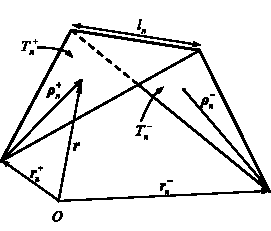
\includegraphics{pica.pdf}
	\caption{RWG 基函数几何参数示意图}
	\label{pica}
\end{figure}
由于时域混合场积分方程是时域电场积分方程与时域磁场积分方程的线性组合,因此时域混合场积分方程时间步进算法的阻抗矩阵特征与时域电场积分方程时间步进算法的阻抗矩阵特征相同。
\begin{equation}
\label{latent_binary_variable}
\mathbf{r}_{i,j}=
\begin{cases}
1,f(\mathbf{x}^{i};\mathbf{w})\cdot f(\mathbf{x}^{j};\mathbf{w})\geq u(\lambda),\\
0,f(\mathbf{x}^{i};\mathbf{w})\cdot f(\mathbf{x}^{j};\mathbf{w})< l(\lambda), 1\leq i,j\leq n.\\
f(\mathbf{x}^{i};\mathbf{w})\cdot f(\mathbf{x}^{j};\mathbf{w}),\text{otherwise},
\end{cases}
\end{equation}

时域积分方程时间步进算法的阻抗元素直接影响算法的后时稳定性,因此阻抗元素的计算是算法的关键之一,采用精度高效的方法计算时域阻抗元素是时域积分方程时间步进算法研究的重点之一。


\subsection{时间基函数}

\subsubsection{时域方法特有的展开函数}

\subsubsection{频域方法特有的展开函数}

\section{入射波}

如图\ref{picb}和图\ref{picc}所示分别给出了参数$E_0=\hat{x}$,$a_n=-\hat{z}$,$f_0=250MHz$,$f_w=50MHz$,$t_w=4.2\sigma$时,调制高斯脉冲的时域与频域归一化波形图。

\begin{figure}[h]
	\subfigure[]{
		\label{picb}
		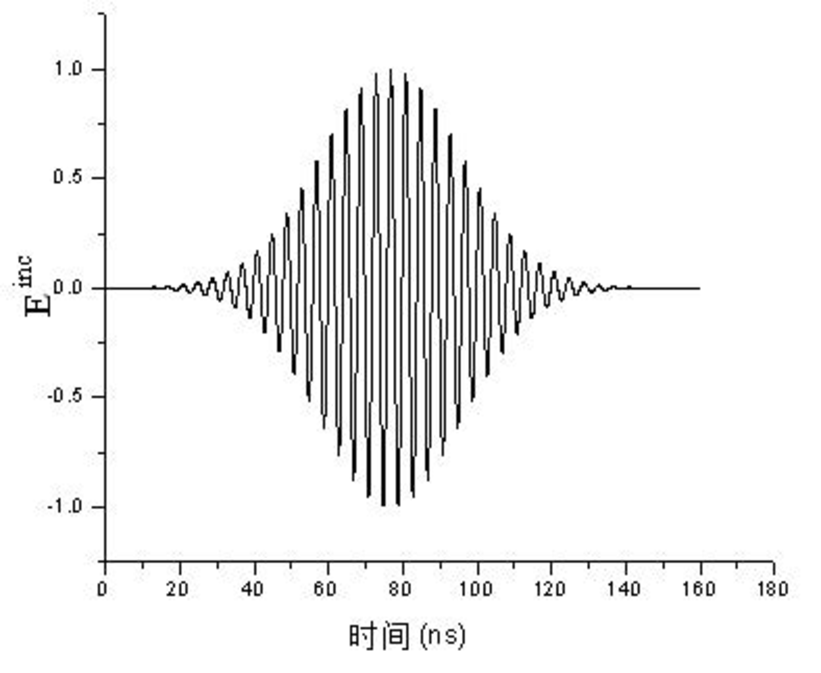
\includegraphics[width=7.3cm]{picb.pdf}}
	\subfigure[]{
		\label{picc}
		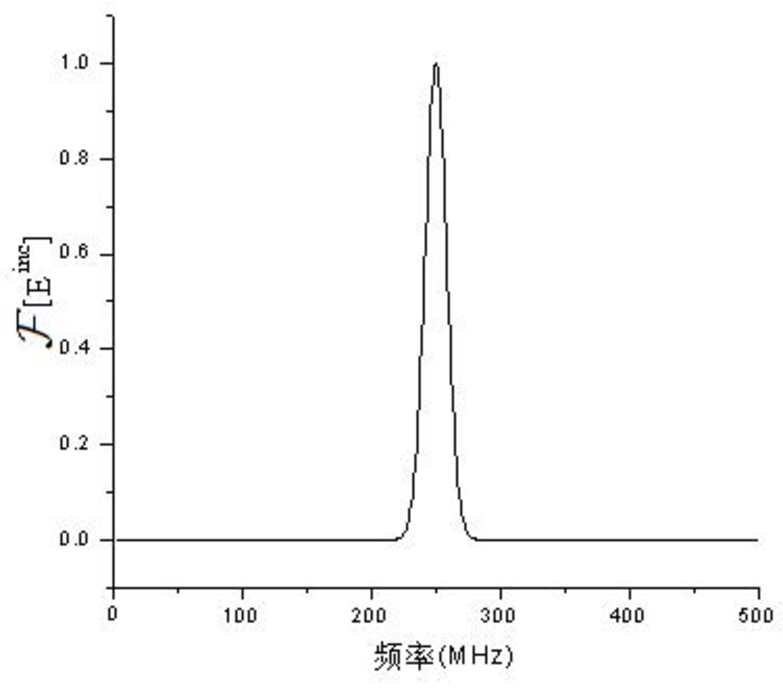
\includegraphics[width=6.41cm]{picc.pdf}}
	\caption{调制高斯脉冲时域与频率波形,时域阻抗元素的存储技术也是时间步进算法并行化的关键技术之一,采用合适的阻抗元素存储方式可以很大的提高并行时间步进算法的计算效率。}
	\label{fig1}
\end{figure}
时域阻抗元素的存储技术\citing{xiao2012yi}也是时间步进算法并行化的关键技术之一,采用合适的阻抗元素存储方式可以很大的提高并行时间步进算法的计算效率。

时域积分方程时间步进算法的阻抗元素直接影响算法的后时稳定性,因此阻抗元素的计算是算法的关键之一,采用精度高效的方法计算时域阻抗元素是时域积分方程时间步进算法研究的重点之一。

\section{时域积分方程时间步进算法阻抗矩阵的存储}
时域阻抗元素的存储技术也是时间步进算法并行化的关键技术之一,采用合适的阻抗元素存储方式可以很大的提高并行时间步进算法的计算效率。

\subsection{时域积分方程时间步进算法产生的阻抗矩阵的特征}
由于时域混合场积分方程是时域电场积分方程与时域磁场积分方程的线性组合,因此时域混合场积分方程时间步进算法的阻抗矩阵特征与时域电场积分方程时间步进算法的阻抗矩阵特征相同。

\subsection{数值算例与分析}

如图3-1(a)所示给出了时间步长选取为0.5ns时采用三种不同存储方式计算的平板中心处 方向的感应电流值与IDFT方法计算结果的比较。如图3-1(b)所示给出了存储方式为基权函数压缩存储方式,时间步长分别取时平板中心处 方向的感应电流计算结果,从图中可以看出不同时间步长的计算结果基本相同。

\begin{algorithm}[H]
	\KwData{this text}
	\KwResult{how to write algorithm with \LaTeX2e }
	initialization\;
	\While{not at end of this document}{
		read current\;
		\eIf{understand}{
			go to next section\;
			current section becomes this one\;
		}{
		go back to the beginning of current section\;
	}
}
\caption{How to wirte an algorithm.}
\end{algorithm}

由于时域混合场积分方程是时域电场积分方程与时域磁场积分方程的线性组合,因此时域混合场积分方程时间步进算法的阻抗矩阵特征与时域电场积分方程时间步进算法的阻抗矩阵特征相同。

\section{时域积分方程时间步进算法矩阵方程的求解}

\section{本章小结}
本章首先研究了时域积分方程时间步进算法的阻抗元素精确计算技术,分别采用DUFFY变换法与卷积积分精度计算法计算时域阻抗元素,通过算例验证了计算方法的高精度。

\end{document}        %第二章
\documentclass{standalone}
% preamble: usepackage, etc.
\begin{document}

\chapter{时域积分方程数值方法研究}
\section{时域积分方程时间步进算法的阻抗元素精确计算}
时域积分方程时间步进算法的阻抗元素直接影响算法的后时稳定性,因此阻抗元素的计算是算法的关键之一,采用精度高效的方法计算时域阻抗元素是时域积分方程时间步进算法研究的重点之一。

% \section{时域积分方程时间步进算法阻抗矩阵的存储}
% 时域阻抗元素的存储技术也是时间步进算法并行化的关键技术之一,采用合适的阻抗元素存储方式可以很大的提高并行时间步进算法的计算效率。

\subsection{时域积分方程时间步进算法产生的阻抗矩阵的特征}
由于时域混合场积分方程是时域电场积分方程与时域磁场积分方程的线性组合,因此时域混合场积分方程时间步进算法的阻抗矩阵特征与时域电场积分方程时间步进算法的阻抗矩阵特征相同。

\subsection{数值算例与分析}

如图3-1(a)所示给出了时间步长选取为0.5ns时采用三种不同存储方式计算的平板中心处 方向的感应电流值与IDFT方法计算结果的比较。如图3-1(b)所示给出了存储方式为基权函数压缩存储方式,时间步长分别取时平板中心处 方向的感应电流计算结果,从图中可以看出不同时间步长的计算结果基本相同。

\begin{algorithm}[H]
	\KwData{this text}
	\KwResult{how to write algorithm with \LaTeX2e }
	initialization\;
	\While{not at end of this document}{
		read current\;
		\eIf{understand}{
			go to next section\;
			current section becomes this one\;
		}{
		go back to the beginning of current section\;
	}
}
\caption{How to wirte an algorithm.}
\end{algorithm}

由于时域混合场积分方程是时域电场积分方程与时域磁场积分方程的线性组合,因此时域混合场积分方程时间步进算法的阻抗矩阵特征与时域电场积分方程时间步进算法的阻抗矩阵特征相同。

\section{时域积分方程时间步进算法矩阵方程的求解}

\section{本章小结}
本章首先研究了时域积分方程时间步进算法的阻抗元素精确计算技术,分别采用DUFFY变换法与卷积积分精度计算法计算时域阻抗元素,通过算例验证了计算方法的高精度。

\end{document}
        %第三章
\documentclass{standalone}
% preamble: usepackage, etc.
\begin{document}

\chapter{时域积分方程数值方法研究}
\section{时域积分方程时间步进算法的阻抗元素精确计算}
时域积分方程时间步进算法的阻抗元素直接影响算法的后时稳定性,因此阻
抗元素的计算是算法的关键之一,采用精度高效的方法计算时域阻抗元素是时域
积分方程时间步进算法研究的重点之一。

\section{时域积分方程时间步进算法阻抗矩阵的存储}
时域阻抗元素的存储技术也是时间步进算法并行化的关键技术之一,采用
合适的阻抗元素存储方式可以很大的提高并行时间步进算法的计算效率。

\subsection{时域积分方程时间步进算法产生的阻抗矩阵的特征}

由于时域混合场积分方程是时域电场积分方程与时域磁场积分方程的线性组
合,因此时域混合场积分方程时间步进算法的阻抗矩阵特征与时域电场积分方程
时间步进算法的阻抗矩阵特征相同。
\subsection{数值算例与分析}
如表\ref{tablea}所示给出了时间步长分别取0.4ns、0.5ns、0.6ns 时的三种存储
方式的存储量大小。

\begin{table}[h]
	\caption{计算$2m\times 2m$理想导体平板时域感应电流采用的三种存储方式的存储量比较。} 
	\begin{tabular}{|c|c|c|c|} 
		\hline  
		时间步长 & 非压缩存储方式 & 完全压缩存储方式 & 基权函数压缩存储方式 \\
		\hline 
		0.4ns & 5.59 MB & 6.78 MB & 6.78 MB\\  
		\hline  
		0.5ns & 10.17 MB & 5.58 MB & 5.58 MB \\  
		\hline  
		0.6ns & 8.38MB & 4.98 MB & 4.98 MB \\  
		\hline  
	\end{tabular}
	\label{tablea}
\end{table}

如图\ref{picd}所示给出了时间步长选取为0.5ns 时采用三种不同存储方式计算的
平板中心处$x$方向的感应电流值与IDFT 方法计算结果的比较,……。如图\ref{pice}
所示给出了存储方式为基权函数压缩存储方式,时间步长分别取0.4ns、0.5ns、0.6ns
时平板中心处$x$方向的感应电流计算结果,从图中可以看出不同时间步长的计算结果基本相同。

由于时域混合场积分方程是时域电场积分方程与时域磁场积分方程的线性组合,因此时域混合场积分方程时间步进算法的阻抗矩阵特征与时域电场积分方程时间步进算法的阻抗矩阵特征相同。

\begin{figure}[h]
	\subfigure[]{
		\label{picd}
		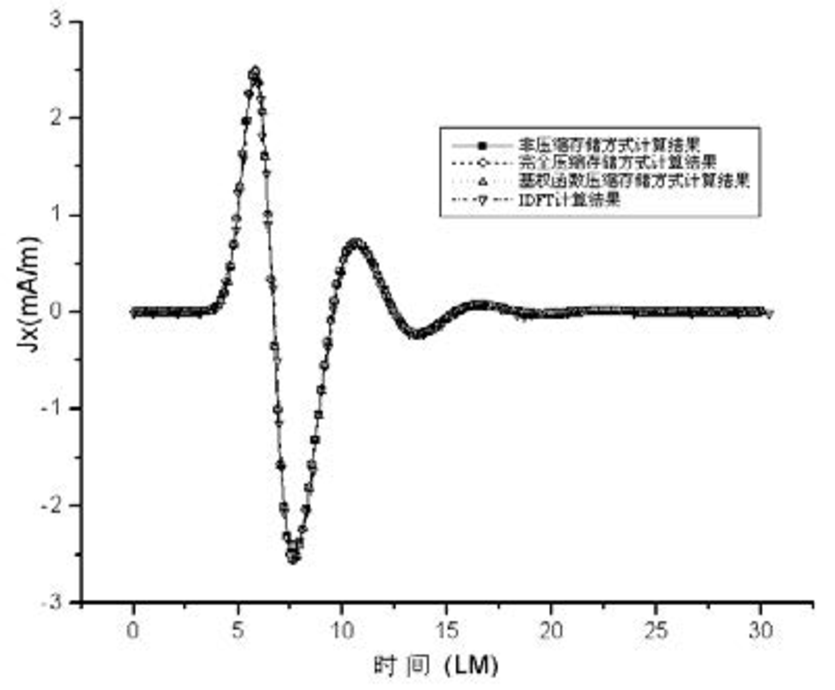
\includegraphics[width=6.77cm]{picd.pdf}}
	\subfigure[]{
		\label{pice}
		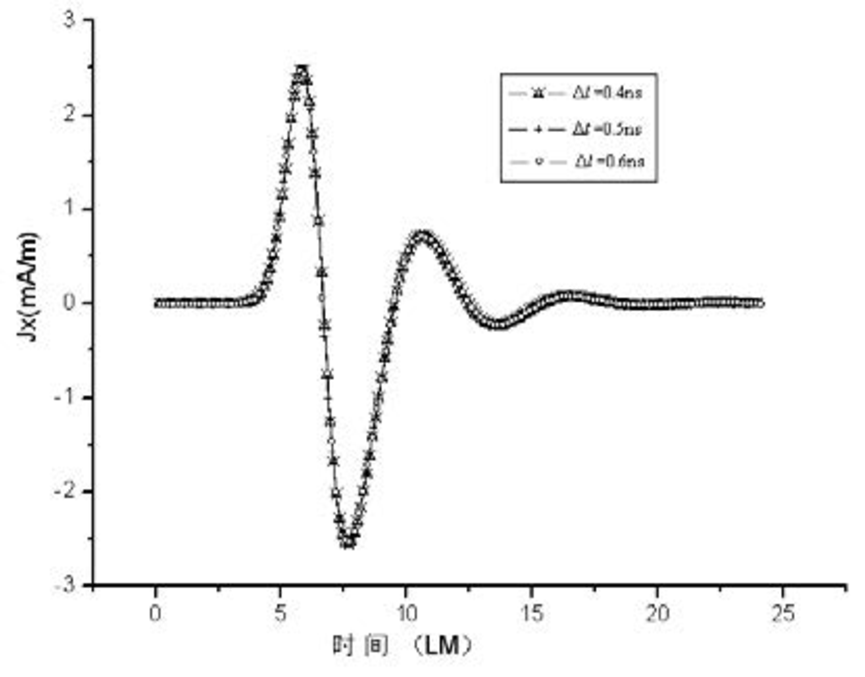
\includegraphics[width=7.04cm]{pice.pdf}}
	\caption{$2m\times 2m$的理想导体平板中心处感应电流$x$分量随时间的变化关系}
	\label{fig2}
\end{figure}


由于时域混合场积分方程是时域电场积分方程与时域磁场积分方程的线性组
合,因此时域混合场积分方程时间步进算法的阻抗矩阵特征与时域电场积分方程
时间步进算法的阻抗矩阵特征相同。
\section{时域积分方程时间步进算法矩阵方程的求解}

\begin{theorem}
	如果时域混合场积分方程是时域电场积分方程与时域磁场积分方程
	的线性组合。
\end{theorem}
\begin{proof}
	由于时域混合场积分方程是时域电场积分方程与时域磁场积分方程的线性组
	合,因此时域混合场积分方程时间步进算法的阻抗矩阵特征与时域电场积分方程
	时间步进算法的阻抗矩阵特征相同。
\end{proof}
\begin{corollary}
	时域积分方程方法的研究近几年发展迅速,在本文研究工作的基础上,仍有以下方向值得进一步研究。
\end{corollary}
\begin{lemma}
	因此时域混合场积分方程时间步进算法的阻抗矩阵特征与时域电场积分方程
	时间步进算法的阻抗矩阵特征相同。
\end{lemma}

\section{本章小结}
本章首先研究了时域积分方程时间步进算法的阻抗元素精确计算技术,分别
采用DUFFY 变换法与卷积积分精度计算法计算时域阻抗元素,通过算例验证了计
算方法的高精度。

\end{document}        %第四章
\documentclass{standalone}
% preamble: usepackage, etc.
\begin{document}
	
\chapter{全文总结与展望}

\section{全文总结}
本文以时域积分方程方法为研究背景,主要对求解时域积分方程的时间步进算法以及两层平面波快速算法进行了研究。

\section{后续工作展望}
时域积分方程方法的研究近几年发展迅速,在本文研究工作的基础上,仍有以下方向值得进一步研究:

\end{document}        %第五章
\documentclass{standalone}
% preamble: usepackage, etc.
\begin{document}
	
\chapter{总结与展望}
\section{全文总结}
本文主要工作是设计和实现了基于一个图同构的初等数学的推理引擎。工作内容主要
分成三个部分:知识图谱构建、实例化定理库构建以及图推理引擎的逻辑结构设计和模块化构建。
知识图谱是知识表示的载体,因此构建一个合理完备的初等数学知识图谱是自然语言理解和自动推理
的关键一步。知识图谱的构建分为实体构建和关系构建,然后将构建的实体类和关系类通过程序化
方式生成对应的图节点和边,存储在neo4j图数据库中。为了实现添加实体类和关系类的可扩展性
和开闭原则,构建了抽象实体类和抽象关系类,所有的实体类都继承于抽象实体类,所有的关系类
都继承于抽象关系类。第二部分是实例化定理库的构建,图推理引擎在推理方式上还是规则引擎
的一种,因此规则库是引擎驱动和产生新知识的重要依据。实例化定理库的构建分为三个环节:
定理收集、定理标准化以及定理实例化。定理收集是原始教材或教辅资料中的定理、公式、公理等描述,
还有一部分是来源于标准答案中的解题过程;完成定理生成后,需要对定理进行规范化、标准化书写,这里
的规范化是指符合推理引擎的定理输入规范格式,方便推理引擎统一处理;定理实例化是将第二环节中的
规范化定理生成知识图谱,存储在规则库中。最后是图推理引擎的整体设计和实现,引擎在架构设计思想上
采用的分层结构,不同逻辑层之间相对独立,模块化程度高;在算法上的核心设计思想是图匹配以及置换
等价问题。最后为了提高引擎的处理问题的能力和稳定性,引入异常检测机制和冲突消解策略。综上可以将
本文中的研究工作及成果分为以下四个要点:

(1)构建了知识图谱中实体类和关系类,并用抽象类的设计思想实现了知识图谱构建的可扩展性,并
定义了抽象类的属性和结构,最终构建的知识图谱实体***********个,关系********条

(2)参与了实例化定理的搜集工作,制定了定理的规范化标准,并完成定理实例化,共
有实例化定理************条

(3)完成了整个推理引擎的设计和构建工作,包括其中的逻辑架构设计和实现,核心算法的设计和实现,
使用的推理方式设计和实现,每层的模块化构建,异常检测机制和冲突消解策略

(4)参与了类人解答过程的算法核心思想设计和部分构建工作。设计类人解答过程的分支回溯思想
,以及推理中的规则树构建。

\section{后续工作展望}
虽然本文完整了整个图推理引擎的设计和构建工作,并且也将推理引擎接入到系统中完成测试工作。
但是引擎在稳定性和兼容性上还存在不足,解题能力也有待提高。由于时间和精力有限,推理引擎中
存在的不足和疑难问题还待解决:

(1)匹配算法的精度问题。目前引擎中使用的匹配粒度是三元组,即三元组是匹配的最小单位。
而三元组采用是类型匹配,当将知识图谱拆成三元组的粒度时,会使图的部分信息丢失。后续工作中
准备采取关联三元组来解决这一问题,让三元组与三元组之间也产生关系依赖。

(2)知识爆炸问题。因为引擎是产生式系统的演变,因此会存在知识迭代,若匹配过程中
出现m个事实对应n个实例化规则模式,将出现组合情况,组合的知识继续参与迭代,迭代次数
过多将出现知识爆炸。后续工作准备在检测机制中加入虚假组合的检测,将无用组合通过检测机制消除掉,
减少知识迭代。

(3)知识冲突问题。推理引擎的第四逻辑层是知识更新,知识更新是完成将新知识插入到原始的知识库中。
当知识库存在于待插入的知识同类型的知识时,会出现知识冲突,如果不解决知识冲突问题,将会导致
知识插入失败,推理迭代出错,甚至会出现推理异常终止。后续工作时继续完善知识冲突消解策略,能够
处理和兼容到更多的知识冲突问题。

(4)推理效率问题。在引擎具备一定的稳定性和兼容性的前提下,需要考虑推理效率问题。
推理效率一般以时间效率和空间效率作为衡量标准。目前系统中影响推理效率主要来源于
三个方面:实例化定理的选取问题、分支组合数、引擎本身的算法。引擎中主要推理方式还是
正向推理,而正向推理是暴力搜索的方式,会出现很多无效匹配;分支组合数过多时,知识迭代
会引起知识爆炸,影响推理效率;引擎的算法需要优化核心的匹配算法。

\end{document}        %第六章

% misc
\documentclass{standalone}
% preamble: usepackage, etc.
\begin{document}

\thesisacknowledgement
在攻读博士学位期间,首先衷心感谢我的导师XXX教授

\end{document}  %致谢
\thesisloadbibliography[nocite]{reference}  %参考文献


% comment while no need
\documentclass{standalone}
% preamble: usepackage, etc.
\begin{document}

\thesisappendix

\end{document}   %附录,论文若无附录则用%将该命令取消
\thesisloadachievement{publications}  %攻读学位期间取得的成果,若无成果则用%将该命令取消
\documentclass{standalone}
% preamble: usepackage, etc.
\begin{document}

\thesistranslationoriginal
\section{A Tight Upper Bound on Bit Error Rate}

\end{document}  %外文资料原文,论文若未引用外文资料则用%将该命令取消
\documentclass{standalone}
% preamble: usepackage, etc.
\begin{document}

\thesistranslationchinese
\section{基于多载波索引键控的正交频分多路复用系统模型}

\end{document}   %外文资料译文,论文若未引用外文资料则用%将该命令取消

\end{document}
